%%%%%%%%%%%%%%%%%%%%%%%%%%%%%%%%%%%%%%%%%%%%%%%%%%%%%%%%%%%%%%%%%%%%%%
% Overleaf (WriteLaTeX) Example: Molecular Chemistry Presentation
%
% Source: http://www.overleaf.com
%
% In these slides we show how Overleaf can be used with standard 
% chemistry packages to easily create professional presentations.
% 
% Feel free to distribute this example, but please keep the referral
% to overleaf.com
% 
%%%%%%%%%%%%%%%%%%%%%%%%%%%%%%%%%%%%%%%%%%%%%%%%%%%%%%%%%%%%%%%%%%%%%%
% How to use Overleaf: 
%
% You edit the source code here on the left, and the preview on the
% right shows you the result within a few seconds.
%
% Bookmark this page and share the URL with your co-authors. They can
% edit at the same time!
%
% You can upload figures, bibliographies, custom classes and
% styles using the files menu.
%
% If you're new to LaTeX, the wikibook is a great place to start:
% http://en.wikibooks.org/wiki/LaTeX
%
%%%%%%%%%%%%%%%%%%%%%%%%%%%%%%%%%%%%%%%%%%%%%%%%%%%%%%%%%%%%%%%%%%%%%%

\documentclass[hyperref={colorlinks,citecolor=blue,linkcolor=blue,urlcolor=blue}]{beamer}

% For more themes, color themes and font themes, see:
% http://deic.uab.es/~iblanes/beamer_gallery/index_by_theme.html
%
\mode<presentation>
{
  \usetheme{Madrid}       % or try default, Darmstadt, Warsaw, ...
  \usecolortheme{default} % or try albatross, beaver, crane, ...
  \usefonttheme{serif}    % or try default, structurebold, ...
  \setbeamertemplate{navigation symbols}{}
  \setbeamertemplate{caption}[numbered]
} 

\usepackage[T2A]{fontenc}
\usepackage[utf8]{inputenc}
\usepackage[english,russian]{babel}
\usepackage{chemfig}
\usepackage[version=3]{mhchem}
\usepackage{svg}

% On Overleaf, these lines give you sharper preview images.
% You might want to `comment them out before you export, though.
\usepackage{pgfpages}
\pgfpagesuselayout{resize to}[%
  physical paper width=8in, physical paper height=6in]

% Here's where the presentation starts, with the info for the title slide
\title{Основные проблемы физики элементарных частиц}
\author{Головинов Георгий}
\institute{МФТИ, 2-304}
\date{16 мая 2024 г.}

\begin{document}

\begin{frame}
  \titlepage
\end{frame}

% These three lines create an automatically generated table of contents.
%\begin{frame}{Краткий план:}
%  \tableofcontents
%\end{frame}

\section{Что мы узнали в течение семестра?}
\subsection{Теория и эксперимент и их взаимосвязь}
\begin{frame}{Введение в теорию}

\begin{itemize}
    \item Знакомство со стандартной моделью
    \begin{itemize}
        \item Основные определения стандартной модели, история ее развития
        \item Предсказывающая сила стандартная модели. Какие явления стандартная модель не описывает?
        \item Возможные расширения стандартной модели
    \end{itemize}
    \item Физика нейтрино 
    \begin{itemize}
        \item Что такое нейтрино? Как они были открыты? Как взаимодействуют с другими частицами?
        \item Явление осцилляции нейтрино
        \item Поиск стерильного нейтрино
        \item Какую роль нейтрино играют в развитии теории?
    \end{itemize}
    \item Экзотические, прелестные частицы
    \item Механизм Хиггса
\end{itemize}

\end{frame}

\begin{frame}{Стандартная модель}
    \begin{figure}[H]
        \centering
        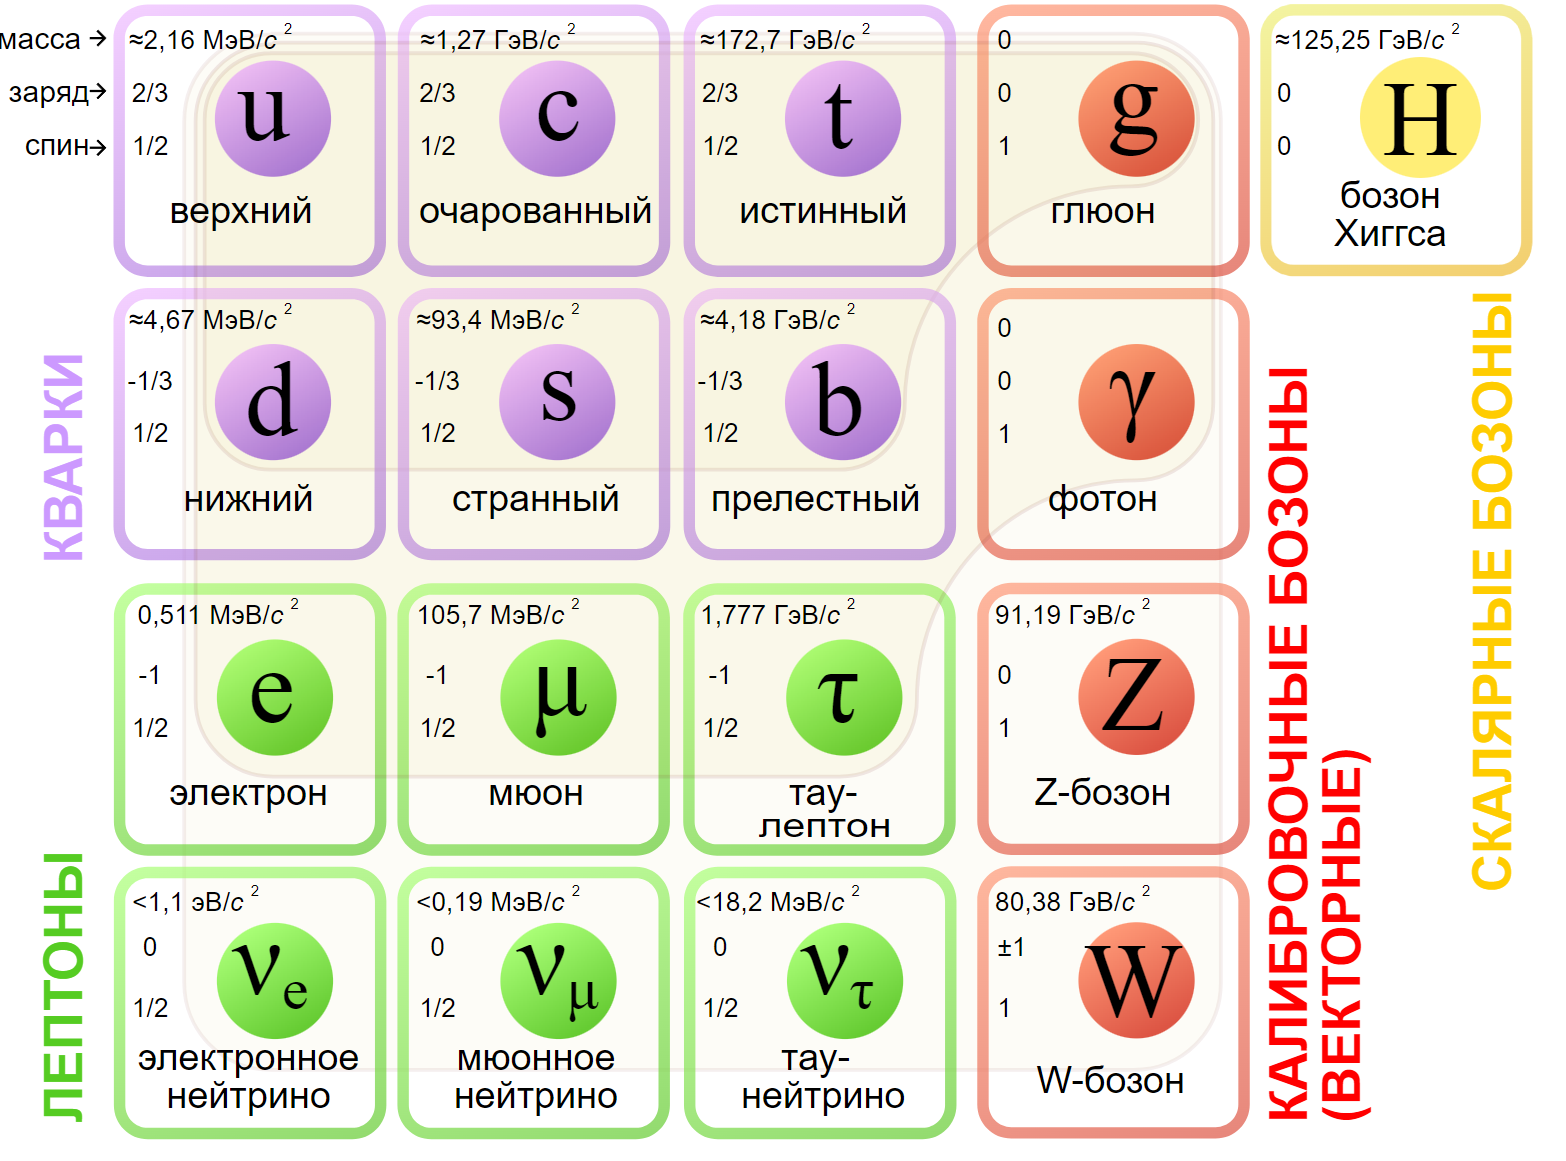
\includegraphics[width=0.7\framewidth]{img/Standard_Model_of_Elementary_Particles_ru.svg.png}
    \end{figure}
    Темная материя? Темная энергия? Масса нейтрино? Масса Хиггса?

\end{frame}

\begin{frame}{Физика нейтрино}
    \begin{block}{Осцилляции нейтрино}
        \begin{equation}
            P(\nu_e\rightarrow\nu_\mu)=\sin^2{2\theta}\sin^2\left(\frac{\Delta m^2 L}{4E}\right)
        \end{equation}
    \end{block}

    %\vspace{0.3cm}

    Есть экспериментальные подтверждения исчезновения или появления $\nu$ на коротких расстояниях $\rightarrow$ возможно объясняется осцилляцией в другое (стерильное) состояние $\rightarrow$ новая физика. 

    %\vspace{0.3cm}
    \textbf{Эксперименты по поиску стерильного нейтрино}
    \begin{figure}[H]
        \centering
        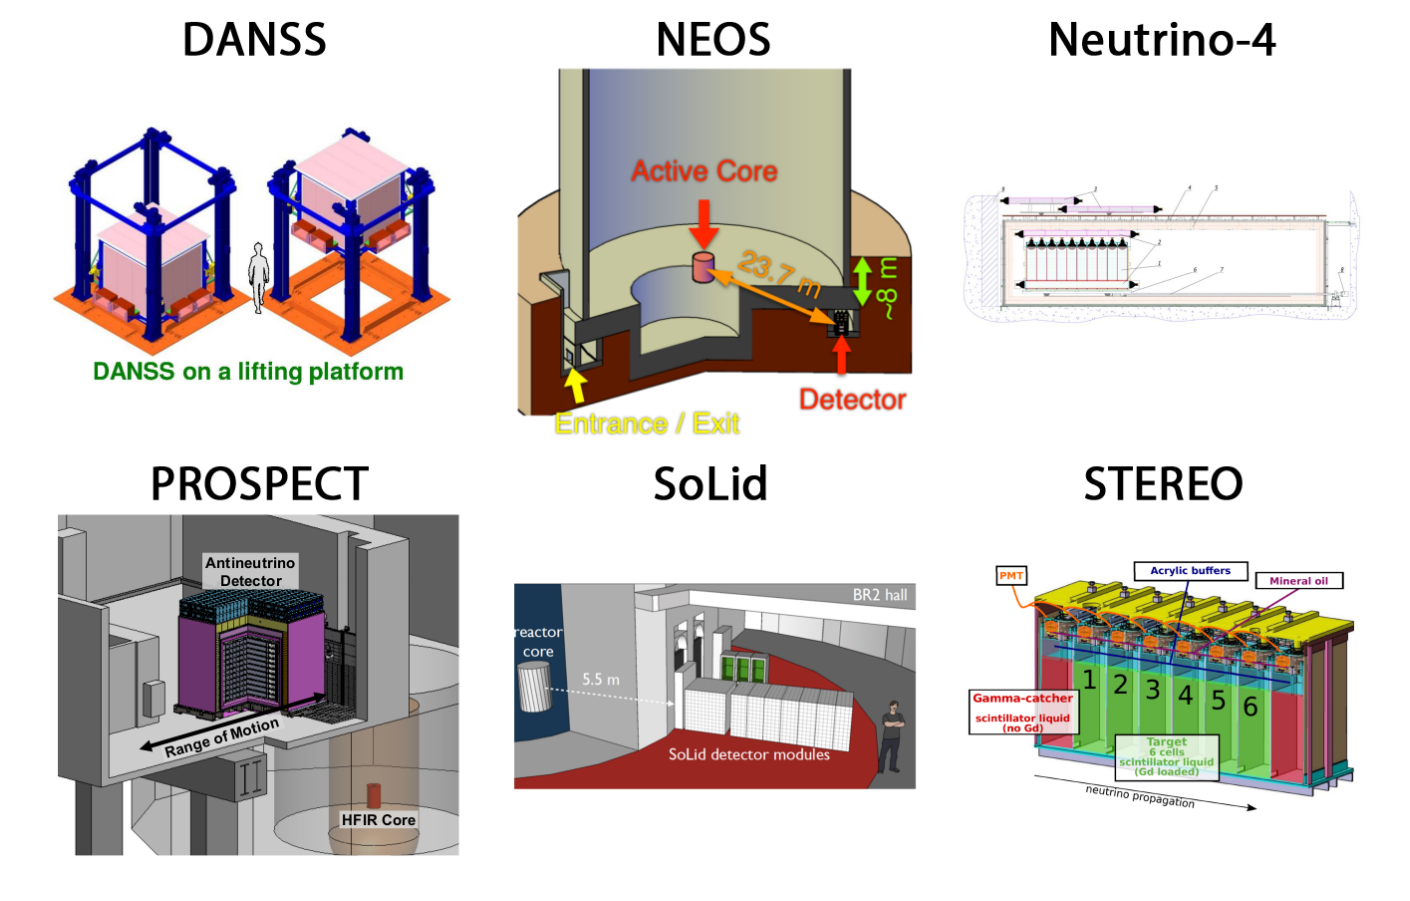
\includegraphics[width=0.5\framewidth]{img/sterile.png}
    \end{figure}
\end{frame}

\begin{frame}{Эксперименты}
    \begin{itemize}
        \item Примеры действующих экспериментов, их цель
        \item Перспективы развития действующих экспериментов
        \item Будущие эксперименты
        \item Как выглядит процесс открытия новых частиц? Как это помогает развитию теории?
        \item Связь теории и эксперимента
    \end{itemize}

\end{frame}


\begin{frame}{LHC}
    \textbf{Эксперимент CMS}
    \begin{figure}[H]
        \centering
        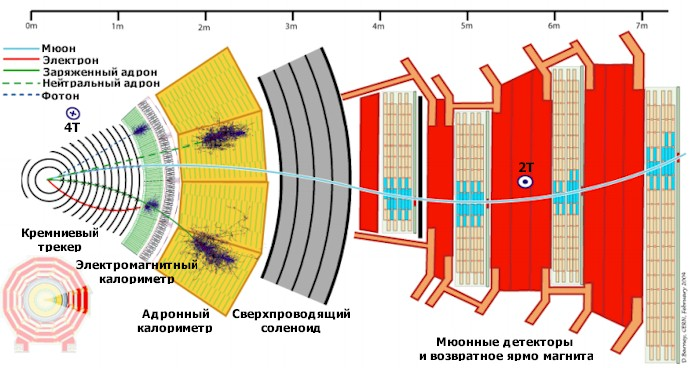
\includegraphics[width=0.7\framewidth]{img/cms02.jpg}
    \end{figure}

\end{frame}

\begin{frame}{NICA}

    \begin{figure}[H]
        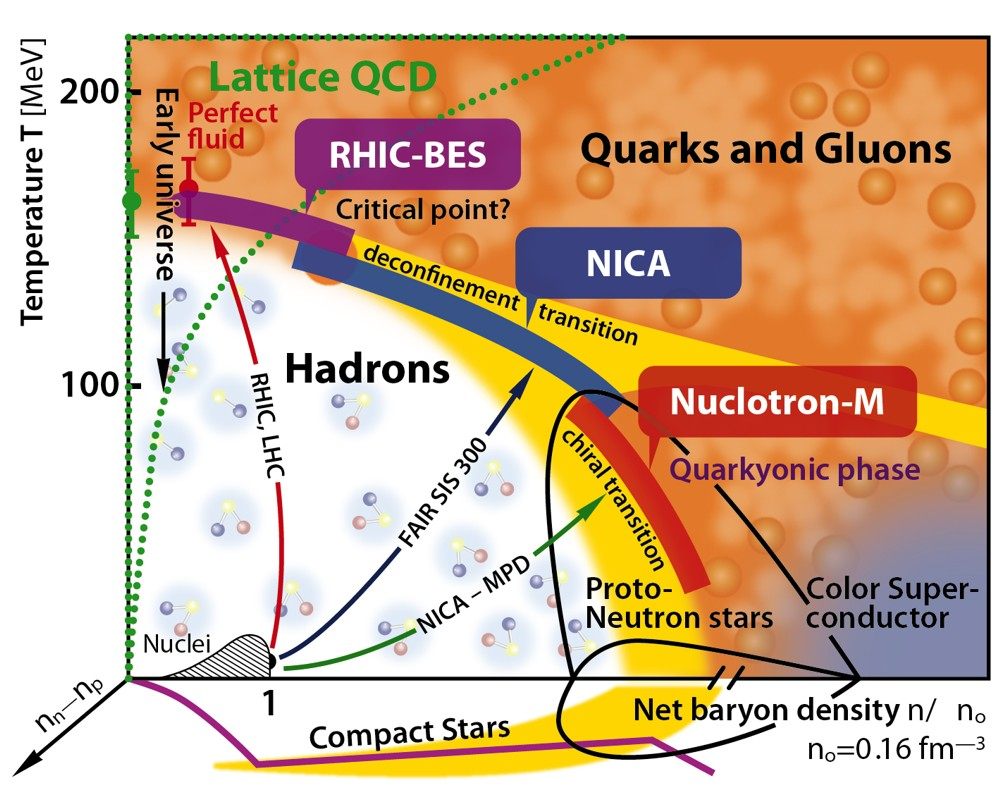
\includegraphics[width=0.7\framewidth]{img/phase.jpg}
    \end{figure}

\end{frame}


\begin{frame}{Что мне понравилось больше всего?}
    Короткий ответ: \textbf{Астрофизика (и физика космоса в целом)}.

    Тесная связь физики космоса и физики элементарных частиц:
    \begin{itemize}
        \item Темная материя, темная энергия и др. --- общие проблемы как физики элементарных частиц, так и физики космоса
        \item Практически любое расширение стандартной модели может в корне изменить представление о развитии вселенной
        \item Физика элементарных частиц сильно влияет на астрофизику: например, при моделировании взрыва сверхновых, если не учитывать вклад нейтрино, то звезды просто перестают взрываться. Если же их учесть, то масса нейтрино (которую мы не знаем) сильно влияет на результат моделирования
        \item Астрофизика уже помогала физике элементарных частиц: многие первые частицы стандартная модели были открыты с помощью космических лучей --- высокоэнергетических частиц из космоса
    \end{itemize}
\end{frame}



\end{document}